\chapter{القوى بين الجزيئات والمذيبات}\label{ch:b1:intermolecular-forces-solvents}

يجري أبو بريص على زجاج نافذة ويتدلى منه بإصبع واحدة؛ بلا غراء ولا
مصّ، بل بمجرد التجاذب بين جزيئات وسائد أصابعه وجزيئات
الزجاج. والماء، وجزيئه أخف من جزيء ثنائي أكسيد الكربون، يغلي
عند \qty{100}{\celsius}، بينما ثنائي أكسيد الكربون غاز في درجة حرارة
الغرفة. والزيت يطفو على الخل ولا يمتزج به أبدًا؛ وملح الطعام
يذوب في الماء ولا يذوب في البنزين. وكل هذه الوقائع لا تحسمها
الروابط داخل الجزيئات، بل القوى الأضعف بكثير بينها. يصنّف هذا الفصل
تلك القوى، ويقيس آثارها في درجات الغليان، ويستعملها لاختيار مذيب.

% ledger: bp:H2O (the hook's 100 degC)

\begin{recall}
قدّم الكتاب الأول (الصف الحادي عشر) قوى فان دير فالس \omterm{def:b1:intermolecular-forces-solvents:hbond}{والروابط الهيدروجينية}،
وبيّن أن الأجسام الصلبة الأيونية تذوب بالتفكك \omterm{def:b1:intermolecular-forces-solvents:dissolution}{والذوبنة}.
وعُرّفت \omterm{def:b1:lewis-resonance-vsepr:dipole}{عزوم ثنائي القطب} في \cref{def:b1:lewis-resonance-vsepr:dipole}
\omterm{def:b1:periodicity:polarisability}{وقابلية الاستقطاب} في \cref{def:b1:periodicity:polarisability}. ونستعمل من
الفيزياء قانون كولوم: شحنتان $q_1$ و$q_2$ على مسافة
$r$ في الفراغ تتجاذبان أو تتنافران بقوة طويلتها $|q_1q_2|/(4\pi
\varepsilon_0 r^2)$.
\end{recall}

\begin{omfigure}
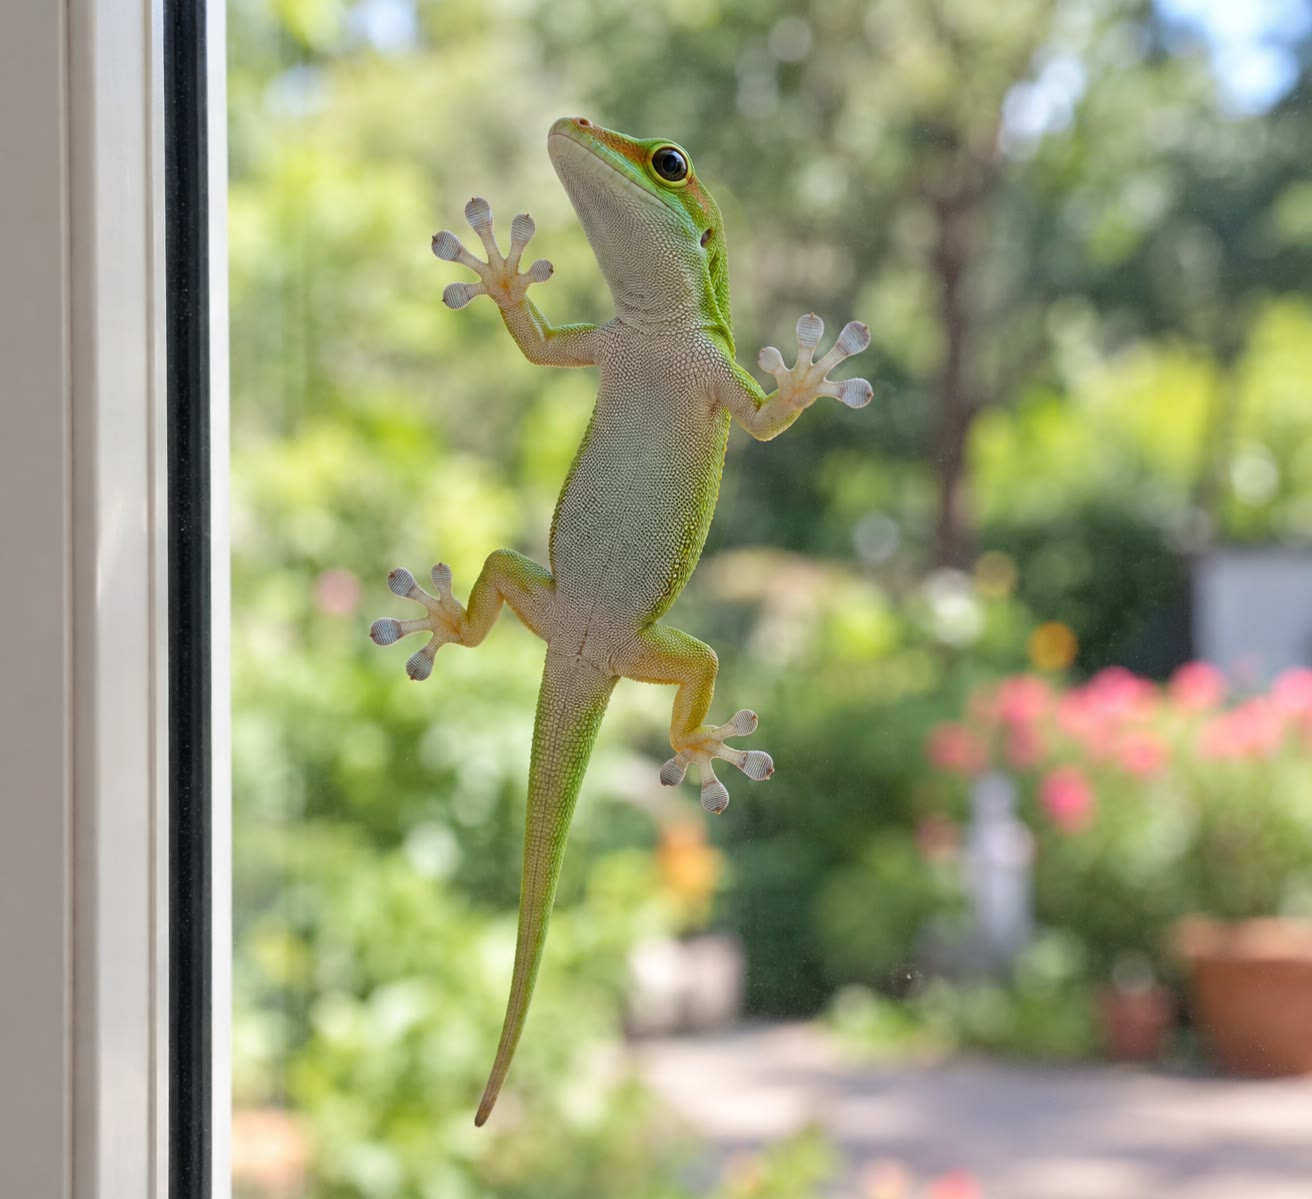
\includegraphics[width=0.52\linewidth]{images/book2/ai/b1-04-gecko.jpg}

{\small أبو بريص على زجاج نافذة. ملايين الشعيرات الدقيقة في وسائد أصابعه
تقترب من الزجاج حتى إن التجاذب الضعيف بين جزيئاتها
وجزيئات الزجاج يتراكم فيفوق وزنه.}
\end{omfigure}

\section{تآثرات فان دير فالس}

\begin{definition}[تآثرات فان دير فالس]\label{def:b1:intermolecular-forces-solvents:vdw}
\emph{تآثرات فان دير فالس}\index{تآثر فان دير فالس}
هي التجاذبات بين الجزيئات المتعادلة الناشئة عن
تآثر ثنائيات أقطابها. ويميَّز منها ثلاثة أنواع:
\begin{itemize}
  \item \emph{تآثر كيسوم}\index{تآثر كيسوم} (أو
        تآثر التوجيه) بين ثنائيي قطب دائمين، يميلان
        إلى الاصطفاف رأسًا إلى ذيل؛
  \item \emph{تآثر ديباي}\index{تآثر ديباي} (أو
        تآثر الحث) بين ثنائي قطب دائم وثنائي القطب
        الذي يحثّه في جار قابل للاستقطاب؛
  \item \emph{تآثر لندن}\index{تآثر لندن} (أو
        تآثر التشتت) بين ثنائيات الأقطاب اللحظية التي تولّدها
        تقلبات السحب الإلكترونية في أي ذرتين أو
        جزيئين، قطبيين أو غير قطبيين، والتي يحث بعضها بعضًا.
\end{itemize}
\end{definition}

\begin{omfigure}
\begin{tikzpicture}[font=\small, >={Stealth},
    mol/.style={draw=black!60, fill=#1, ellipse, minimum width=1.5cm, minimum height=0.8cm}]
  % Keesom
  \node[mol=omDef!20] (a) at (0,0) {}; \node[mol=omDef!20] (b) at (1.7,0) {};
  \node at (-0.45,0) {$\delta^-$}; \node at (0.45,0) {$\delta^+$};
  \node at (1.25,0) {$\delta^-$}; \node at (2.15,0) {$\delta^+$};
  \node[below, align=center] at (0.85,-0.65) {\foreignlanguage{arabic}{كيسوم:}\\ثنائيا قطب دائمان};
  % Debye
  \begin{scope}[xshift=4.6cm]
    \node[mol=omDef!20] at (0,0) {}; \node[mol=black!5, dashed] at (1.7,0) {};
    \node at (-0.45,0) {$\delta^-$}; \node at (0.45,0) {$\delta^+$};
    \node[omProp] at (1.25,0) {$\delta^-$}; \node[omProp] at (2.15,0) {$\delta^+$};
    \node[below, align=center] at (0.85,-0.65) {\foreignlanguage{arabic}{ديباي:}\\دائم ومحثوث};
  \end{scope}
  % London
  \begin{scope}[xshift=9.2cm]
    \node[mol=black!5, dashed] at (0,0) {}; \node[mol=black!5, dashed] at (1.7,0) {};
    \node[omProp] at (-0.45,0) {$\delta^-$}; \node[omProp] at (0.45,0) {$\delta^+$};
    \node[omProp] at (1.25,0) {$\delta^-$}; \node[omProp] at (2.15,0) {$\delta^+$};
    \node[below, align=center] at (0.85,-0.65) {\foreignlanguage{arabic}{لندن:}\\ثنائيا قطب لحظيان};
  \end{scope}
\end{tikzpicture}

{\small \omterm{def:b1:intermolecular-forces-solvents:vdw}{تآثرات فان دير فالس} الثلاثة. الشحنات الجزئية السوداء
دائمة (\omterm{def:b1:lewis-resonance-vsepr:dipole}{جزيئات قطبية})؛ والبرتقالية محثوثة أو لحظية.
وفي كل حالة تكون الشحنتان المتقابلتان متعاكستين، فتتجاذب
الجزيئات.}
\end{omfigure}

\begin{proposition}[الشدة والمدى]\label{prop:b1:intermolecular-forces-solvents:distance-law}
من أجل جزيئين على مسافة $r$، تتغير كل طاقة من طاقات فان دير فالس
الثلاث كما $-1/r^6$: فلا يُحس التجاذب إلا بين
الجيران. وطاقاتها من رتبة بضعة كيلوجولات لكل
مول، أي أقل بنحو مئة مرة من طاقة \omterm{def:b1:lewis-resonance-vsepr:lewis}{رابطة تساهمية}. ويكبر حد لندن
مع قابليتي الاستقطاب لدى الشريكين؛ وهو حاضر
بين كل الجزيئات وهو عادةً أكبر الثلاثة، إلا
في الجزيئات الصغيرة الشديدة القطبية.
\end{proposition}
\admitted

\begin{example}[الغازات النبيلة والهالوجينات]\label{ex:b1:intermolecular-forces-solvents:noble}
لا تتجاذب ذرات الغاز النبيل إلا بقوى لندن،
التي تكبر مع عدد الإلكترونات: يغلي الهيليوم عند
\qty{-268.9}{\celsius}، والنيون عند \qty{-246.1}{\celsius}، والأرغون عند
\qty{-185.9}{\celsius}، والكريبتون عند \qty{-153.4}{\celsius}، والزينون عند
\qty{-108.1}{\celsius}. وكذلك يكون ثنائي الفلور وثنائي الكلور، في درجة حرارة الغرفة،
غازين، وثنائي البروم سائلًا (يغلي عند \qty{58.8}{\celsius})
وثنائي اليود جسمًا صلبًا.
% ledger: bp:He, bp:Ne, bp:Ar, bp:Kr, bp:Xe, bp:F2, bp:Cl2, bp:Br2, bp:I2
\end{example}

\begin{omfigure}
\begin{tikzpicture}
\begin{axis}[
  width=0.62\linewidth, height=5.4cm,
  xmin=0.5, xmax=10.5, ymin=-180, ymax=200,
  axis x line=bottom, axis y line=left,
  xlabel={\foreignlanguage{arabic}{عدد ذرات الكربون $n$}}, ylabel={\foreignlanguage{arabic}{درجة الغليان \babelsublr{(\unit{\celsius})}}},
  xtick={1,2,3,4,5,6,7,8,9,10}, ytick={-150,-100,-50,0,50,100,150},
  tick label style={font=\small}, label style={font=\small}]
\addplot[omDef, thick, mark=*, mark size=1.5pt] table[x=n, y=bp_C] {figdata/out/bachelor-1-hydride-boiling-points-alkanes.dat};
\end{axis}
\end{tikzpicture}

{\small درجات غليان الألكانات الخطية \ce{C_nH_{2n+2}}، من الميثان إلى
الديكان. كل مجموعة \ce{CH2} مضافة تضيف إلكترونات وسطح تماس، ومن ثم
تجاذب لندن؛ وتتناقص الزيادة ببطء، من نحو
\qty{75}{\celsius} في البداية إلى \qty{25}{\celsius} عند الديكان.}
\end{omfigure}

\section{الرابطة الهيدروجينية}

\begin{definition}[الرابطة الهيدروجينية]\label{def:b1:intermolecular-forces-solvents:hbond}
\emph{الرابطة الهيدروجينية}\index{رابطة هيدروجينية} تجاذب
$\ce{X-H}\cdots\ce{Y}$ بين ذرة هيدروجين مرتبطة بذرة صغيرة شديدة
\omterm{def:b1:periodicity:electronegativity}{الكهرسلبية} X (\ce{N} أو \ce{O} أو \ce{F}) \omterm{def:b1:lewis-resonance-vsepr:lewis}{وزوج حر}
لذرة كهرسلبية أخرى Y. والجزيء الحامل للرابطة \ce{X-H} هو
مانح الرابطة الهيدروجينية، والحامل للذرة Y هو مستقبلها. وطاقتها، من 10
إلى \qty{40}{kJ/mol}، تقع بين طاقات \omterm{def:b1:intermolecular-forces-solvents:vdw}{تآثرات فان دير فالس} وطاقات \omterm{def:b1:lewis-resonance-vsepr:lewis}{الروابط
التساهمية}؛ والذرات الثلاث \ce{X} و\ce{H} و\ce{Y} شبه مصطفّة.
\end{definition}

\begin{remark}[لماذا N وO وF]\label{rem:b1:intermolecular-forces-solvents:why}
تترك X الشديدة \omterm{def:b1:periodicity:electronegativity}{الكهرسلبية} للهيدروجين شحنة جزئية موجبة
كبيرة؛ والهيدروجين، الذي لا \omterm{def:b1:quantum-numbers:configuration}{إلكترونات داخلية} له، ضئيل الحجم، فيستطيع
\omterm{def:b1:lewis-resonance-vsepr:lewis}{الزوج الحر} للذرة Y أن يقترب منه كثيرًا. والشرطان لازمان كلاهما:
فالروابط \ce{C-H} ليست قطبية بما يكفي، والروابط \ce{S-H} أو \ce{Cl-H}
تضم ذرات أكبر مما ينبغي وأضعف كهرسلبية من أن تكوّن \omterm{def:b1:intermolecular-forces-solvents:hbond}{روابط هيدروجينية}
قوية.
\end{remark}

\begin{omfigure}
\begin{tikzpicture}[font=\small]
  % water network
  \foreach \n/\x/\y/\a in {1/0/0/0, 2/2.2/0.9/200, 3/0.2/-2.0/60, 4/-2.1/0.6/-30} {
    \begin{scope}[shift={(\x,\y)}, rotate=\a]
      \node[aO] (o\n) at (0,0) {};
      \node[aH] (h\n a) at (0.78,0.3) {};
      \node[aH] (h\n b) at (-0.2,-0.82) {};
      \begin{scope}[on background layer]
        \draw[bond] (o\n.center) -- (h\n a.center); \draw[bond] (o\n.center) -- (h\n b.center);
      \end{scope}
    \end{scope}
  }
  \draw[omThm, thick, densely dotted] (h1a) -- (o2);
  \draw[omThm, thick, densely dotted] (h1b) -- (o3);
  \draw[omThm, thick, densely dotted] (h4a) -- (o1);
  \node[below] at (0,-2.9) {الماء: كل جزيء يمكنه أن يمنح اثنتين ويستقبل اثنتين};
  % carboxylic acid dimer
  \begin{scope}[xshift=5.6cm, yshift=-0.6cm]
    \node (r1) at (-0.9,0) {R}; \node (c1) at (0,0) {C};
    \node (o1) at (0.6,0.85) {O}; \node (o2) at (0.6,-0.85) {O}; \node (h2) at (1.45,-0.85) {H};
    \node (c2) at (3.3,0) {C}; \node (r2) at (4.2,0) {R};
    \node (o3) at (2.7,0.85) {O}; \node (o4) at (2.7,-0.85) {O}; \node (h3) at (1.85,0.85) {H};
    \draw (r1) -- (c1) -- (o2) -- (h2) (c2) -- (r2) (c2) -- (o3) -- (h3);
    \draw[double, double distance=1.6pt] (c1) -- (o1); \draw[double, double distance=1.6pt] (c2) -- (o4);
    \draw[omThm, thick, densely dotted] (h2) -- (o4) (h3) -- (o1);
    \node[below] at (1.65,-2.3) {مثنوي حمض كربوكسيلي};
  \end{scope}
\end{tikzpicture}

{\small \omterm{def:b1:intermolecular-forces-solvents:hbond}{الروابط الهيدروجينية} (منقّطة بالأحمر). في الماء السائل يشارك كل جزيء
في ما يصل إلى أربع منها؛ وتتزاوج الأحماض الكربوكسيلية في مثنويات حلقية
تمسكها \omterm{def:b1:intermolecular-forces-solvents:hbond}{رابطتان هيدروجينيتان}.}
\end{omfigure}

\begin{proposition}[الروابط الهيدروجينية ترفع درجات الغليان]\label{prop:b1:intermolecular-forces-solvents:hbond-bp}
بين هيدريدات الزمر 15 و16 و17، تتزايد درجة الغليان
من \omterm{def:b1:periodicity:table}{الدورة} 3 إلى الدورة 5، تبعًا \omterm{def:b1:intermolecular-forces-solvents:vdw}{لتآثر لندن}؛ أما هيدريدات
\omterm{def:b1:periodicity:table}{الدورة} 2، \ce{NH3} و\ce{H2O} و\ce{HF}، التي تكوّن \omterm{def:b1:intermolecular-forces-solvents:hbond}{روابط
هيدروجينية}، فتغلي فوق امتداد ذلك المنحى بكثير. وهيدريدات
\omterm{def:b1:periodicity:table}{الزمرة} 14 (\ce{CH4} و\ce{SiH4} و\ce{GeH4}) لا تكوّن \omterm{def:b1:intermolecular-forces-solvents:hbond}{روابط هيدروجينية}
وتتبع المنحى.
\end{proposition}

\begin{omfigure}
\begin{tikzpicture}
\begin{axis}[
  width=0.82\linewidth, height=6.6cm,
  xmin=1.5, xmax=5.6, ymin=-180, ymax=120,
  axis x line=bottom, axis y line=left,
  xlabel={الدورة}, ylabel={\foreignlanguage{arabic}{درجة الغليان \babelsublr{(\unit{\celsius})}}},
  xtick={2,3,4,5}, ytick={-150,-100,-50,0,50,100},
  tick label style={font=\small}, label style={font=\small},
  clip=false]
\addplot[black!60, thick, mark=square*, mark size=1.6pt] table[x=period, y=bp_C] {figdata/out/bachelor-1-hydride-boiling-points-g14.dat};
\addplot[omDef, thick, mark=*, mark size=1.6pt] table[x=period, y=bp_C] {figdata/out/bachelor-1-hydride-boiling-points-g15.dat};
\addplot[omThm, thick, mark=*, mark size=1.6pt] table[x=period, y=bp_C] {figdata/out/bachelor-1-hydride-boiling-points-g16.dat};
\addplot[omMeth, thick, mark=triangle*, mark size=2pt] table[x=period, y=bp_C] {figdata/out/bachelor-1-hydride-boiling-points-g17.dat};
\addplot[omThm, dashed] coordinates {(2,-79.3) (3,-60.3)};
\node[font=\small, anchor=west] at (axis cs:2.05,100) {\ce{H2O}};
\node[font=\small, anchor=west] at (axis cs:2.05,19.6) {\ce{HF}};
\node[font=\small, anchor=west] at (axis cs:2.05,-30) {\ce{NH3}};
\node[font=\small, anchor=east] at (axis cs:1.96,-162) {\ce{CH4}};
\node[font=\small, anchor=west] at (axis cs:4.05,-41.3) {\ce{H2Se}};
\node[font=\small, anchor=west] at (axis cs:5.05,-18.4) {\ce{SbH3}};
\node[font=\small, anchor=west] at (axis cs:5.05,-35.1) {\ce{HI}};
\node[font=\small, anchor=west] at (axis cs:4.05,-88.1) {\ce{GeH4}};
\node[font=\small, omThm, anchor=north west] at (axis cs:2.05,-85) {بالاستكمال};
\end{axis}
\end{tikzpicture}

{\small درجات غليان هيدريدات \omterm{def:b1:periodicity:table}{الزمرة} 14 (مربعات رمادية)، و15
(بالأزرق)، و16 (بالأحمر)، و17 (بالأخضر). كان الماء سيغلي قرب
\qty{-79}{\celsius} لو تبع نظائره الأثقل (الخط المتقطع)؛ وروابطه
الهيدروجينية ترفعها بنحو \qty{180}{\celsius}.}
% ledger: bp:CH4, bp:SiH4, bp:GeH4, bp:NH3, bp:PH3, bp:AsH3, bp:SbH3,
% bp:H2O, bp:H2S, bp:H2Se, bp:HF, bp:HCl, bp:HBr, bp:HI
\end{omfigure}

\begin{example}[الإيثانول ومتماكبه]\label{ex:b1:intermolecular-forces-solvents:isomers}
للإيثانول، \ce{CH3CH2OH}، وللميثوكسي ميثان، \ce{CH3OCH3}، الصيغة نفسها
\ce{C2H6O} وتآثرات لندن نفسها تقريبًا. فالإيثانول،
الذي مجموعته \ce{O-H} مانحة ومستقبلة معًا، يغلي عند
\qty{78.4}{\celsius}؛ أما الميثوكسي ميثان، الذي لا يستطيع إلا أن يستقبل، فيغلي عند
\qty{-25.0}{\celsius}.
% ledger: bp:C2H5OH, bp:CH3OCH3
\end{example}

\section{المذيبات}

\begin{definition}[السماحية النسبية]\label{def:b1:intermolecular-forces-solvents:permittivity}
في وسط ما، تُقسم قوة كولوم بين شحنتين على عدد
$\varepsilon_r \ge 1$، هو \emph{السماحية النسبية}\index{سماحية نسبية}
(أو ثابت العزل الكهربائي) للوسط:
\[
  F = \frac{|q_1 q_2|}{4\pi\varepsilon_0\varepsilon_r r^2} .
\]
وهي كبيرة في سوائل \omterm{def:b1:lewis-resonance-vsepr:dipole}{الجزيئات القطبية}، التي تتوجه حول
الشحنات فتحجبها: \num{78.4} للماء عند \qty{25}{\celsius}،
و\num{1.89} للهكسان عند \qty{20}{\celsius}.
% ledger: epsr:H2O, epsr:C6H14
\end{definition}

\begin{definition}[المذيبات القطبية والبروتونية واللابروتونية]\label{def:b1:intermolecular-forces-solvents:solvent-classes}
\emph{المذيب القطبي}\index{مذيب قطبي} مكوّن من جزيئات ذات
\omterm{def:b1:lewis-resonance-vsepr:dipole}{عزم ثنائي قطب} كبير وله \omterm{def:b1:intermolecular-forces-solvents:permittivity}{سماحية نسبية} كبيرة (أكثر من نحو
15)؛ والمذيب غير القطبي سماحيته صغيرة. و\emph{المذيب
البروتوني}\index{مذيب بروتوني} جزيئاته تحمل ذرات هيدروجين
قادرة على تكوين \omterm{def:b1:intermolecular-forces-solvents:hbond}{روابط هيدروجينية} (\ce{O-H} أو \ce{N-H})؛ و\emph{المذيب
اللابروتوني}\index{مذيب لابروتوني} لا يحمل أيًّا منها.
\end{definition}

\begin{center}
\small
\begin{tabular}{lccll}
\hline
المذيب & $\varepsilon_r$ & $\mu$ (D) & القطبية & البروتونية \\
\hline
الماء & 78.4 & 1.86 & قطبي & بروتوني \\
الميثانول & 32.6 & 1.67 & قطبي & بروتوني \\
الإيثانول & 24.3 & 1.52 & قطبي & بروتوني \\
الأسيتونتريل، \ce{CH3CN} & 37.5 & 3.92 & قطبي & لابروتوني \\
البروبانون (الأسيتون) & 20.7 & 2.88 & قطبي & لابروتوني \\
ثنائي كلورو الميثان & 9.08 & 1.62 & ضعيف القطبية & لابروتوني \\
إيثانوات الإيثيل & 6.02 & 1.78 & ضعيف القطبية & لابروتوني \\
الإيثوكسي إيثان & 4.34 & 1.15 & ضعيف القطبية & لابروتوني \\
البنزين & 2.28 & 0 & غير قطبي & لابروتوني \\
الهكسان & 1.89 & 0 & غير قطبي & لابروتوني \\
\hline
\end{tabular}
\end{center}
% ledger: epsr:H2O, epsr:CH3OH, epsr:C2H5OH, epsr:CH3CN, epsr:CH3COCH3,
% epsr:CH2Cl2, epsr:EtOAc, epsr:Et2O, epsr:C6H6, epsr:C6H14, dip:H2O,
% dip:CH3OH, dip:C2H5OH, dip:CH3CN, dip:CH3COCH3, dip:CH2Cl2, dip:EtOAc,
% dip:Et2O, dip:C6H6 (relative permittivities at 20 or 25 degC; dipole
% moments of the gas-phase molecules; hexane has no dipole by symmetry)

\begin{definition}[الذوبنة، القدرة المؤيِّنة والقدرة المفكِّكة]\label{def:b1:intermolecular-forces-solvents:dissolution}
\emph{ذوبنة}\index{ذوبنة} جسيم مذاب هي
إحاطته بجزيئات مذيب متوجهة ومرتبطة به بقوى
بين جزيئية (وهي الإماهة في الماء). و\emph{القدرة
المؤيِّنة}\index{قدرة مؤيِّنة} لمذيب هي قدرته على تحويل
\omterm{def:b1:lewis-resonance-vsepr:lewis}{رابطة تساهمية} قطبية في المذاب إلى زوج أيونات، وهي خاصية
\omterm{def:b1:intermolecular-forces-solvents:solvent-classes}{المذيبات القطبية} ذات \omterm{def:b1:lewis-resonance-vsepr:dipole}{عزم ثنائي القطب} الكبير؛ و\emph{القدرة
المفكِّكة}\index{قدرة مفكِّكة} هي قدرته على فصل أيوني
الزوج، وتقاس بسماحيته النسبية.
\end{definition}

\begin{proposition}[الذوبان في ثلاث خطوات]\label{prop:b1:intermolecular-forces-solvents:steps}
يمكن وصف ذوبان إلكتروليت في مذيب بثلاث
خطوات: التأين (لمذاب جزيئي مثل \ce{HCl})، وتفكك
أزواج الأيونات، \omterm{def:b1:intermolecular-forces-solvents:dissolution}{وذوبنة} الأيونات المنفصلة. ويُذيب المذيب
المذابَ الأيوني أو الشديد القطبية جيدًا حين يكون قطبيًا (مؤيِّنًا)، عالي
السماحية (مفكِّكًا) وقادرًا على \omterm{def:b1:intermolecular-forces-solvents:dissolution}{ذوبنة} الأيونين كليهما --- الكاتيونات
بأزواجه الحرة، والأنيونات \omterm{def:b1:intermolecular-forces-solvents:hbond}{بروابط هيدروجينية} إن كان بروتونيًا.
والماء يفعل الثلاثة.
\end{proposition}

\begin{example}[كلوريد الهيدروجين في الماء وفي الهكسان]\label{ex:b1:intermolecular-forces-solvents:hcl}
في الماء يتأين \ce{HCl} ويتفكك تمامًا:
\ce{HCl(g) + H2O(l) -> H3O+(aq) + Cl-(aq)}؛ فيوصل المحلول التيار. وفي
الهكسان، غير القطبي والمنخفض السماحية، يذوب على هيئة جزيئات \ce{HCl}
ولا يوصل المحلول التيار.
\end{example}

\begin{omfigure}
\begin{tikzpicture}[font=\small]
  \node[aNa] (na) at (0,0) {};
  \node[font=\scriptsize, white] at (na) {\ce{Na+}};
  \foreach \a in {0,60,...,300} {
    \begin{scope}[shift={(\a:1.25)}, rotate=\a]
      \node[aO] (o) at (0,0) {};
      \node[aH] (ha) at (0.55,0.5) {}; \node[aH] (hb) at (0.55,-0.5) {};
      \begin{scope}[on background layer]
        \draw[bond] (o.center) -- (ha.center); \draw[bond] (o.center) -- (hb.center);
      \end{scope}
    \end{scope}
  }
  \node[below] at (0,-2.4) {الكاتيون: أزواج الأكسجين الحرة نحو الداخل};
  \begin{scope}[xshift=6.2cm]
    \node[aCl] (cl) at (0,0) {};
    \node[font=\scriptsize, white] at (cl) {\ce{Cl-}};
    \foreach \a in {0,60,...,300} {
      \begin{scope}[shift={(\a:1.55)}, rotate=\a]
        \node[aH] (h1) at (-0.62,0) {};
        \node[aO] (o) at (0,0) {};
        \node[aH] (h2) at (0.25,0.72) {};
        \begin{scope}[on background layer]
          \draw[bond] (o.center) -- (h1.center); \draw[bond] (o.center) -- (h2.center);
        \end{scope}
      \end{scope}
    }
    \node[below] at (0,-2.4) {الأنيون: الروابط الهيدروجينية نحو الداخل};
  \end{scope}
\end{tikzpicture}

{\small إماهة أيوني كلوريد الصوديوم (الطبقة الأولى وحدها،
مرسومة في المستوي). يوجّه الماء طرفه السالب، الأكسجين، نحو
الكاتيون، وإحدى ذرتي هيدروجينه نحو الأنيون.}
\end{omfigure}

\section{الذوبانية والامتزاج والجزيئات المحبة للوسطين}

\begin{proposition}[الشبيه يذيب الشبيه]\label{prop:b1:intermolecular-forces-solvents:like}
يذوب المذاب جيدًا في مذيب حين تكون التآثرات بين جزيئات المذاب
وجزيئات المذيب مماثلة لتلك التي تفقدها: المذابات القطبية أو
المكوّنة للأيونات في \omterm{def:b1:intermolecular-forces-solvents:solvent-classes}{المذيبات القطبية}، والمذابات غير القطبية في المذيبات
غير القطبية، والمذابات المكوّنة \omterm{def:b1:intermolecular-forces-solvents:hbond}{لروابط هيدروجينية} في \omterm{def:b1:intermolecular-forces-solvents:solvent-classes}{المذيبات البروتونية}.
\end{proposition}

\begin{proof}[استدلال]
يكسر الذوبان تآثرات مذاب--مذاب ومذيب--مذيب
ويكوّن تآثرات مذاب--مذيب. فإذا كان المذاب غير قطبي والمذيب ماءً،
فقدت جزيئات الماء \omterm{def:b1:intermolecular-forces-solvents:hbond}{روابط هيدروجينية} لتفسح له مكانًا ولم تكسب
مقابلها إلا تآثرات لندن ضعيفة: فالذوبان غير مواتٍ. وإذا
كانا كلاهما غير قطبيين، تقاربت تآثرات لندن المفقودة والمكتسبة،
ورجّح الخلطَ الاضطرابُ الذي يحدثه.
\end{proof}

\begin{definition}[السوائل القابلة للامتزاج]\label{def:b1:intermolecular-forces-solvents:miscibility}
يكون سائلان \emph{قابلين للامتزاج}\index{قابل للامتزاج} حين يمتزجان بكل
النسب في طور سائل واحد؛ وإلا كوّنا طبقتين،
الأقل كثافة منهما في الأعلى.
\end{definition}

\begin{example}[الماء مع الإيثانول، والماء مع الهكسان]\label{ex:b1:intermolecular-forces-solvents:miscible}
الإيثانول \omterm{def:b1:intermolecular-forces-solvents:miscibility}{قابل للامتزاج} بالماء: كلاهما بروتوني وقطبي، والإيثانول
يكوّن \omterm{def:b1:intermolecular-forces-solvents:hbond}{روابط هيدروجينية} مع الماء كما يكوّنها مع نفسه. أما الهكسان والماء
فغير \omterm{def:b1:intermolecular-forces-solvents:miscibility}{قابلين للامتزاج}. وثنائي اليود، وهو جسم صلب جزيئي، قليل الذوبان جدًا في الماء لكنه
يذوب بسهولة في الهكسان أو في ثنائي كلورو الميثان: فإذا رُجّ اليود المائي مع مذيب
كهذا انتقل إلى الطبقة العضوية، وهذا مبدأ
الاستخلاص سائل--سائل (\cref{ch:b1:lab-techniques-1}).
\end{example}

\begin{omfigure}
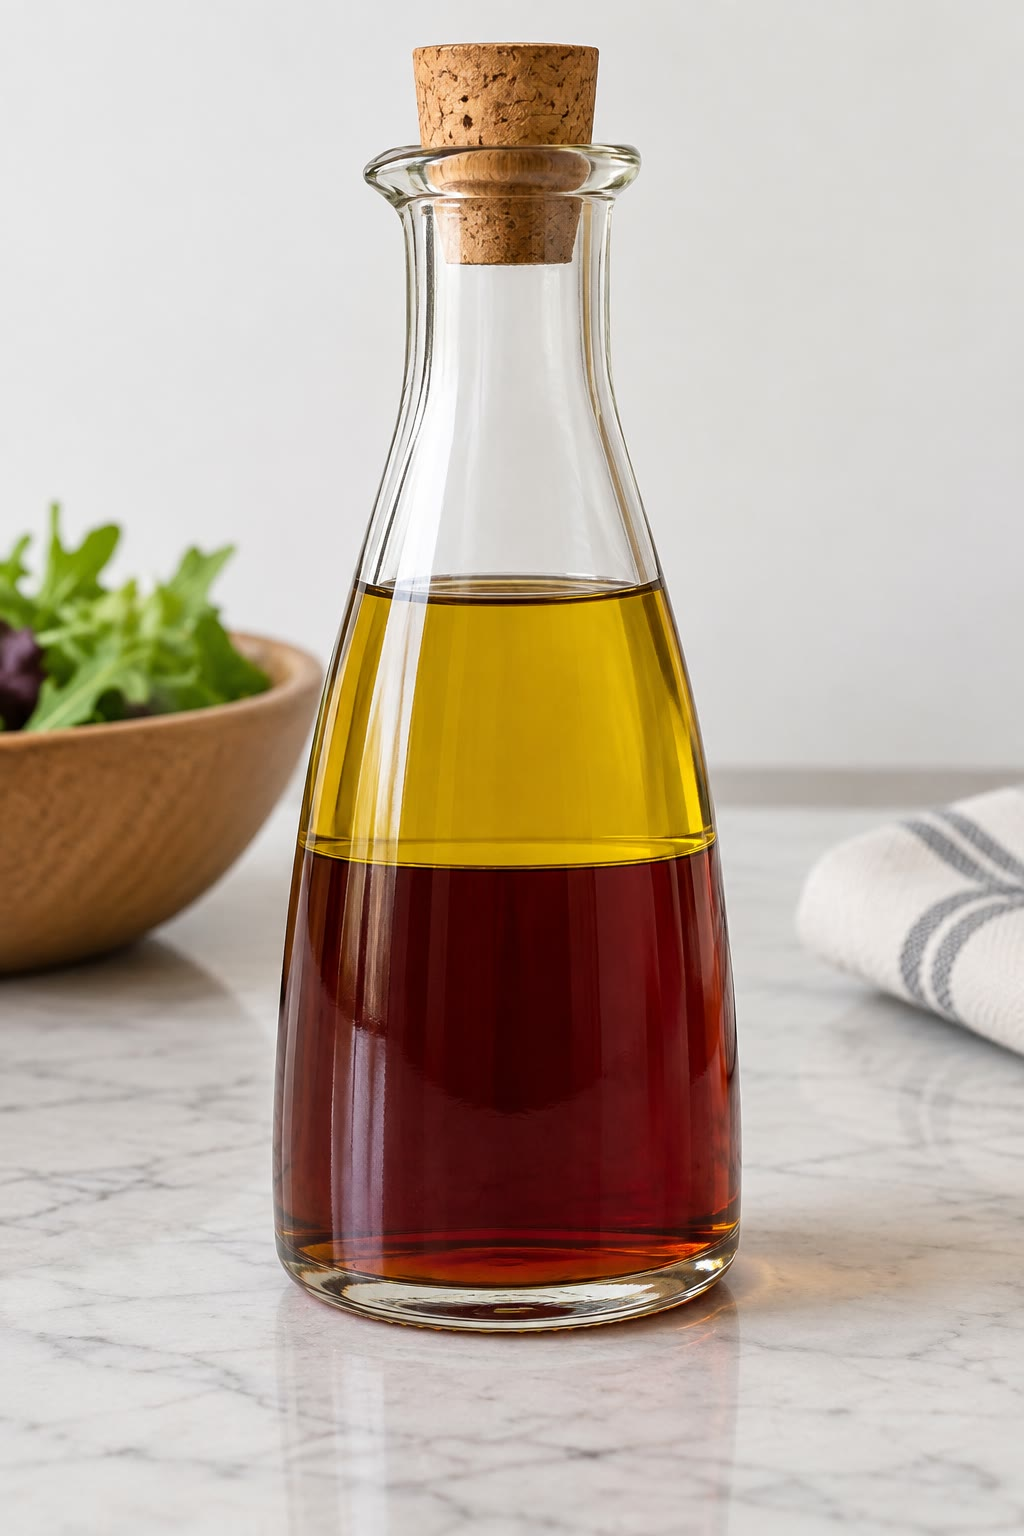
\includegraphics[width=0.2\linewidth]{images/book2/ai/b1-04-dressing.jpg}

{\small صلصة سلطة في حالة سكون: زيت الزيتون، غير القطبي، يطفو على الخل،
وهو محلول مائي؛ والسائلان غير \omterm{def:b1:intermolecular-forces-solvents:miscibility}{قابلين للامتزاج}.}
\end{omfigure}

\begin{definition}[المحب للماء، الكاره للماء، المحب للوسطين]\label{def:b1:intermolecular-forces-solvents:amphiphile}
تكون المجموعة \emph{محبة للماء}\index{محب للماء} حين تتآثر
تآثرًا مواتيًا مع الماء (مجموعات أيونية أو قطبية: \ce{-COO^-}، \ce{-OH}،
\ce{-SO3^-}) و\emph{كارهة للماء}\index{كاره للماء} حين لا تتآثر
(السلاسل الهيدروكربونية). ويكون الجزيء \emph{محبًّا للوسطين}\index{محب للوسطين}
حين يحمل رأسًا محبًا للماء وذيلًا كارهًا للماء معًا.
\end{definition}

\begin{example}[الصابون]\label{ex:b1:intermolecular-forces-solvents:soap}
دوديكانوات الصوديوم، \ce{CH3(CH2)10COO- Na+}، محبة للوسطين. فعند
سطح الماء تنتصب جزيئاتها والرأس في الماء
والذيل في الهواء. وفي باطن السائل، فوق تركيز صغير، تتجمع
في كرات --- هي المذيلات --- ذيولها في الداخل ورؤوسها
في الخارج. والدهن، غير القطبي، يذوب في القلب \omterm{def:b1:intermolecular-forces-solvents:amphiphile}{الكاره للماء} للمذيلات
ويحمله الماء بعيدًا.
\end{example}

\begin{omfigure}
\begin{tikzpicture}[font=\small]
  % interface
  \fill[omWater] (-3.2,-1.6) rectangle (-0.4,0);
  \draw[omDef!60] (-3.2,0) -- (-0.4,0);
  \node[anchor=south west] at (-3.2,0.95) {الهواء};
  \node[anchor=north west] at (-3.2,-1.2) {الماء};
  \foreach \x in {-2.9,-2.5,...,-0.6} {
    \fill[omThm] (\x,-0.12) circle (0.11);
    \draw[thick, black!70, decorate, decoration={zigzag, amplitude=1pt, segment length=3pt}] (\x,0) -- (\x,0.85);
  }
  % micelle
  \begin{scope}[xshift=3.2cm, yshift=-0.4cm]
    \fill[omWater] (-2,-1.6) rectangle (2,1.6);
    \foreach \a in {0,30,...,330} {
      \draw[thick, black!70, decorate, decoration={zigzag, amplitude=1pt, segment length=3pt}] (\a:0.25) -- (\a:1.0);
      \fill[omThm] (\a:1.12) circle (0.11);
    }
    \node[anchor=north] at (0,-1.65) {مذيلة في الماء};
  \end{scope}
\end{tikzpicture}

{\small جزيئات محبة للوسطين (رأس أحمر \omterm{def:b1:intermolecular-forces-solvents:amphiphile}{محب للماء}، وذيل متعرج \omterm{def:b1:intermolecular-forces-solvents:amphiphile}{كاره
للماء}) عند سطح الماء ومتجمعة في مذيلة، مرسومة في
مقطع عرضي؛ وتُدرس المذيلات في مجلد السنة الثالثة.}
\end{omfigure}

\begin{method}[اختيار مذيب]\label{met:b1:intermolecular-forces-solvents:choose}
لاختيار مذيب لمذاب أو لتفاعل:
\begin{enumerate}
  \item حدّد طبيعة المذاب: أيوني، أو قطبي، أو قادر على منح \omterm{def:b1:intermolecular-forces-solvents:hbond}{روابط
        هيدروجينية} أو استقبالها، أو غير قطبي؛
  \item اختر مذيبًا من النوع نفسه (\cref{prop:b1:intermolecular-forces-solvents:like})،
        عالي السماحية إن وجب فصل أيونات؛
  \item لتفاعل بين أنيون وجزيء، فضّل مذيبًا قطبيًا
        لابروتونيًا، يذيب الملح دون أن يربط
        الأنيون \omterm{def:b1:intermolecular-forces-solvents:hbond}{بروابط هيدروجينية} (\cref{ch:b1:nucleophilic-substitution})؛
  \item للاستخلاص، اختر مذيبًا غير \omterm{def:b1:intermolecular-forces-solvents:miscibility}{قابل للامتزاج} بالمذيب الأول
        ويذوب فيه المذاب أكثر بكثير.
\end{enumerate}
\end{method}

\section{تمارين}

\begin{exercise}[$\star$]\label{exo:b1:intermolecular-forces-solvents:1}
سمِّ التآثرات القائمة بين جسيمات الأرغون السائل،
وكلوريد الهيدروجين السائل، والماء السائل، والميثان السائل، وثنائي اليود
الصلب، وبيّن أيها الغالب في كل حالة.
\end{exercise}

\begin{exercise}[$\star$]\label{exo:b1:intermolecular-forces-solvents:2}
أي هذه المواد يكوّن \omterm{def:b1:intermolecular-forces-solvents:hbond}{روابط هيدروجينية} بين جزيئاته
نفسها: \ce{CH3OH}، \ce{CH3OCH3}، \ce{CH3NH2}، \ce{CH3F}، \ce{HF}،
\ce{CH4}؟ وأيها لا يستطيع إلا أن يستقبل \omterm{def:b1:intermolecular-forces-solvents:hbond}{روابط هيدروجينية} من جزيء آخر؟
\end{exercise}

\begin{exercise}[$\star$]\label{exo:b1:intermolecular-forces-solvents:3}
مستعينًا بجدول المذيبات، صنّف الماء والإيثانول والبروبانون والهكسان
وثنائي كلورو الميثان والأسيتونتريل إلى قطبية أو غير قطبية، وبروتونية أو لابروتونية.
\end{exercise}

\begin{exercise}[$\star$]\label{exo:b1:intermolecular-forces-solvents:4}
فسّر لماذا يذوب ثنائي اليود في الهكسان أفضل بكثير منه في الماء،
ولماذا يفعل كلوريد الصوديوم العكس.
\end{exercise}

\begin{exercise}[$\star\star$]\label{exo:b1:intermolecular-forces-solvents:5}
يغلي الميثانول عند \qty{64.7}{\celsius}، والإيثانول عند \qty{78.4}{\celsius}،
وحمض الإيثانويك عند \qty{118.1}{\celsius} والميثوكسي ميثان عند
\qty{-25.0}{\celsius}. فسّر هذا الترتيب.
% ledger: bp:CH3OH, bp:C2H5OH, bp:CH3COOH, bp:CH3OCH3
\end{exercise}

\begin{exercise}[$\star\star$]\label{exo:b1:intermolecular-forces-solvents:6}
احسب قوة كولوم بين أيون \ce{Na+} وأيون \ce{Cl-}
تفصل بينهما \qty{500}{pm} في الفراغ ($\varepsilon_0 = \qty{8.854e-12}{F/m}$،
$e = \qty{1.602e-19}{C}$)، ثم في الماء ($\varepsilon_r = 78.4$) وفي
الهكسان ($\varepsilon_r = 1.89$). علّق.
\end{exercise}

\begin{exercise}[$\star\star$]\label{exo:b1:intermolecular-forces-solvents:7}
البروبانون والماء قابلان للامتزاج بكل النسب؛ أما الهكسان والماء
فلا. فسّر، مراعيًا التآثرات المكسورة والمتكوّنة.
\end{exercise}

\begin{exercise}[$\star\star$]\label{exo:b1:intermolecular-forces-solvents:8}
لجزيء \ce{HCl} \omterm{def:b1:lewis-resonance-vsepr:dipole}{عزم ثنائي قطب} \qty{1.09}{\debye} ويغلي عند
\qty{-85.0}{\celsius}؛ ولجزيء \ce{HBr} عزم \qty{0.83}{\debye} ويغلي عند
\qty{-66.4}{\celsius}. لماذا يغلي الجزيء الأقل قطبية عند درجة أعلى؟
% ledger: dip:HCl, dip:HBr, bp:HCl, bp:HBr
\end{exercise}

\begin{exercise}[$\star\star$]\label{exo:b1:intermolecular-forces-solvents:9}
ارسم المثنوي الحلقي لحمض الإيثانويك. في محلول البنزين يسلك حمض
الإيثانويك كأن كتلته المولية نحو ضعف \qty{60}{g/mol}؛ أما في
الماء فلا. فسّر الواقعتين.
\end{exercise}

\begin{exercise}[$\star\star\star$]\label{exo:b1:intermolecular-forces-solvents:10}
صف ذوبان كلوريد الصوديوم في الماء بلغة
التفكك \omterm{def:b1:intermolecular-forces-solvents:dissolution}{والذوبنة}، وذوبان كلوريد الهيدروجين في الماء بلغة
التأين والتفكك \omterm{def:b1:intermolecular-forces-solvents:dissolution}{والذوبنة}. ولماذا يعطي كلوريد
الهيدروجين في الهكسان محلولًا غير موصل؟
\end{exercise}

\begin{exercise}[$\star\star\star$]\label{exo:b1:intermolecular-forces-solvents:11}
انطلاقًا من درجات غليان الألكانات الخطية (البنتان
\qty{36.1}{\celsius}، والديكان \qty{174.1}{\celsius})، احسب متوسط
الزيادة لكل مجموعة \ce{CH2} بين \ce{C5} و\ce{C10}، وقدّر
درجة غليان الأونديكان. لماذا تتناقص الزيادة على امتداد
السلسلة؟
% ledger: bp:C5H12, bp:C10H22
\end{exercise}

\begin{exercise}[$\star\star\star$]\label{exo:b1:intermolecular-forces-solvents:12}
دوديسيل كبريتات الصوديوم، \ce{CH3(CH2)11OSO3^- Na+}، منظِّف. عيّن
جزأيه \omterm{def:b1:intermolecular-forces-solvents:amphiphile}{المحب للماء} \omterm{def:b1:intermolecular-forces-solvents:amphiphile}{والكاره للماء}، وارسم ترتيبه عند
سطح الماء وفي مذيلة، وفسّر كيف يزيل بقعة
زيتية من نسيج.
\end{exercise}

\section{مسألة: لو لم تكن للماء روابط هيدروجينية}

\begin{problem}[{مسألة نهاية الأسبوع --- قوى لندن في الغازات النبيلة
والألكانات، واختيار مذيب، ودرجة الغليان التي كانت للماء
لولا الروابط الهيدروجينية}]
\label{pb:b1:intermolecular-forces-solvents:1}
درجات الغليان تحت \qty{1}{atm} (بالوحدة \unit{\celsius}): \ce{He} $-268.9$،
\ce{Ne} $-246.1$، \ce{Ar} $-185.9$، \ce{Kr} $-153.4$، \ce{Xe} $-108.1$؛
البنتان 36.1، والهكسان 68.8؛ \ce{CH4} $-161.5$، \ce{SiH4} $-112.0$،
\ce{GeH4} $-88.1$؛ \ce{NH3} $-33.4$، \ce{PH3} $-87.8$، \ce{AsH3} $-62.5$؛
\ce{H2O} 100.0، \ce{H2S} $-60.3$، \ce{H2Se} $-41.3$؛ \ce{HF} 19.6،
\ce{HCl} $-85.0$، \ce{HBr} $-66.4$.
% ledger: bp:He, bp:Ne, bp:Ar, bp:Kr, bp:Xe, bp:C5H12, bp:C6H14, bp:CH4,
% bp:SiH4, bp:GeH4, bp:NH3, bp:PH3, bp:AsH3, bp:H2O, bp:H2S, bp:H2Se,
% bp:HF, bp:HCl, bp:HBr

\medskip
\noindent\textbf{الجزء الأول --- لندن وحده.}
\begin{enumerate}
  \item أي تآثر يمسك ذرات الأرغون السائل بعضها ببعض؟
  \item فسّر تزايد درجة الغليان من الهيليوم إلى الزينون.
  \item لماذا كانت درجة غليان الهيليوم أدنى درجات غليان المواد كلها؟
  \item قارن البنتان بالهكسان: ماذا تضيف مجموعة \ce{CH2} واحدة؟
  \item ليس للميثان والسيلان والجيرمان \omterm{def:b1:lewis-resonance-vsepr:dipole}{عزم ثنائي قطب}. أي
        تآثر يفسر ترتيب درجات غليانها؟
  \item لماذا لا تمكن أي \omterm{def:b1:intermolecular-forces-solvents:hbond}{رابطة هيدروجينية} في الميثان؟
\end{enumerate}

\medskip
\noindent\textbf{الجزء الثاني --- اختيار المذيبات.}
استعمل جدول المذيبات الوارد في الفصل.
\begin{enumerate}[resume]
  \item أي مذيب في الجدول يذيب كلوريد الصوديوم أفضل من غيره،
        ولماذا؟
  \item بأي عامل يكون التجاذب بين أيونين أصغر في
        الماء منه في الهكسان على المسافة نفسها؟
  \item ينبغي إجراء تفاعل بين الأنيون \ce{CN-} وجزيء عضوي
        في مذيب يذيب الملح لكنه لا
        يربط الأنيون \omterm{def:b1:intermolecular-forces-solvents:hbond}{بروابط هيدروجينية}. اختر واحدًا.
  \item لاستخلاص ثنائي اليود من محلول مائي، أي مذيب في
        الجدول تختار، وفي أي طبقة ينتهي اليود؟
  \item فسّر لماذا لا يمكن استعمال الإيثانول في هذا الاستخلاص.
  \item الإيثوكسي إيثان قليل الامتزاج بالماء مع أنه قطبي.
        اقترح تفسيرًا.
\end{enumerate}

\medskip
\noindent\textbf{الجزء الثالث --- الهيدريدات الأخرى.}
\begin{enumerate}[resume]
  \item في \omterm{def:b1:periodicity:table}{الزمرة} 17، احسب تغير درجة الغليان من \ce{HCl} إلى
        \ce{HBr}، ومدّد التغير نفسه رجوعًا إلى الدورة 2.
  \item قارن القيمة المستكمَلة بدرجة غليان \ce{HF}.
  \item السؤالان نفسهما \omterm{def:b1:periodicity:table}{للزمرة} 15 (\ce{PH3} و\ce{AsH3}
        و\ce{NH3}).
  \item في \omterm{def:b1:periodicity:table}{الزمرة} 14، هل يقع \ce{CH4} فوق الاستكمال
        من \ce{SiH4} و\ce{GeH4} أم تحته؟ ولماذا لا يدعو ذلك إلى الاستغراب؟
  \item رتّب فوائض \ce{NH3} و\ce{HF} والماء.
  \item عُدّ \omterm{def:b1:intermolecular-forces-solvents:hbond}{الروابط الهيدروجينية} التي يستطيع كل جزيء من \ce{NH3} و\ce{HF}
        و\ce{H2O} أن يمنحها ويستقبلها، وفسّر الترتيب.
\end{enumerate}

\medskip
\noindent\textbf{الجزء الرابع --- ماء بلا \omterm{def:b1:intermolecular-forces-solvents:hbond}{روابط هيدروجينية}.}
\begin{enumerate}[resume]
  \item لماذا يصلح \ce{H2S} و\ce{H2Se} للاستكمال،
        ولماذا لا يصلح الماء نفسه؟
  \item احسب تغير درجة الغليان من \ce{H2S} إلى \ce{H2Se}.
  \item اكتب معادلة المستقيم المار بهاتين النقطتين،
        ومتغيره \omterm{def:b1:periodicity:table}{الدورة} $p$.
  \item استنتج درجة الغليان التي تكون للماء عند $p = 2$.
  \item بكم ترفع \omterm{def:b1:intermolecular-forces-solvents:hbond}{الروابط الهيدروجينية} درجة غليان الماء؟
  \item استنتج: عند أي درجة حرارة كان الماء سيغلي لو تجاذبت جزيئاته
        كما تتجاذب جزيئات \ce{H2S}؟
\end{enumerate}
\end{problem}
